\selectlanguage{australian}%

\chapter{Results}

\acresetall


\section{Humanly Perceived Improvement vs. Machine Performance}


\subsection{Investigating Existing Data}

The direct comparison method outlined in \subsecref{Method-Existing-Data}
was carried out on the data given in \secref{litresults} \textit{\nameref{sec:litresults}}.
The R code used to perform this analysis is given in \lstref{directComp}.

\figref{Direct-PESQ-PRR} shows the results obtained, comparing the
\ac{PESQ} improvement against the \ac{PRR} improvement. \figref{Direct-PESQ-PRR-LOESS}
shows the data fitted with an \ac{LOESS} model and \figref{Direct-PESQ-PRR-LM}
shows the data fitted with an \ac{LM} method.

\begin{figure}[h]
\subfloat[\label{fig:Direct-PESQ-PRR-LOESS}\acs{LOESS} fit]{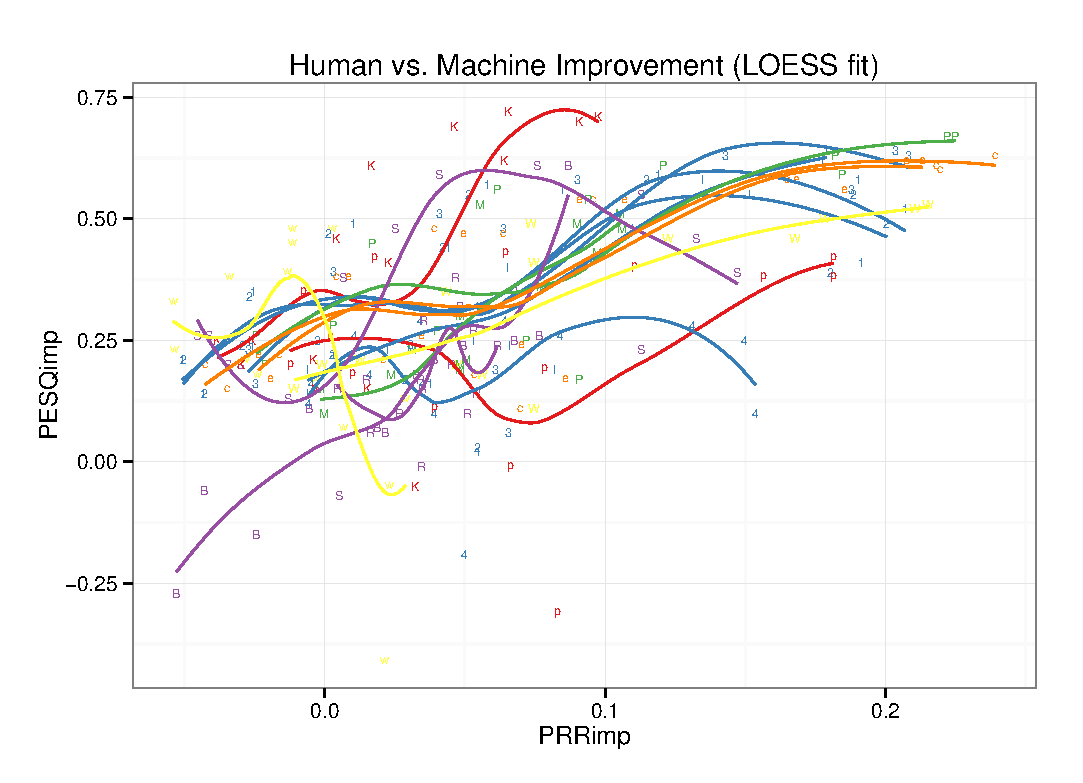
\includegraphics[width=1\textwidth]{fig/R/dir/HumanMachineAllLOESS}

}

\subfloat[\label{fig:Direct-PESQ-PRR-LM}\acl{LM} fit]{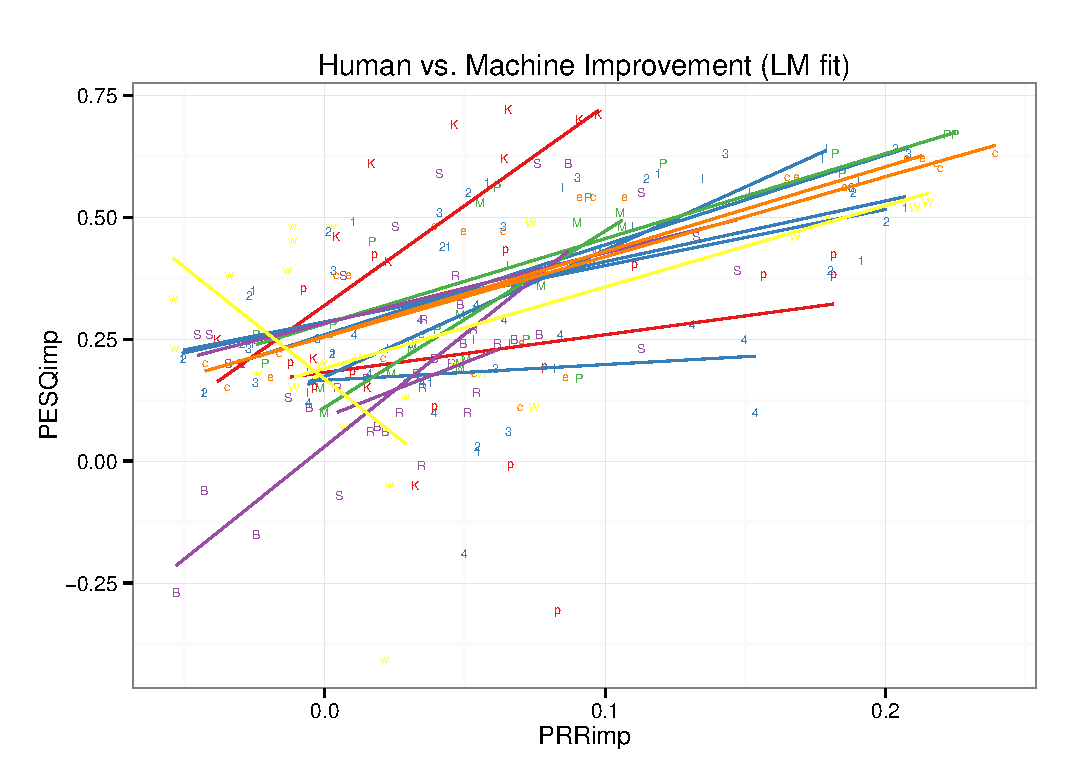
\includegraphics[width=0.8\textwidth]{fig/R/dir/HumanMachineAllLM}\includegraphics[width=0.2\textwidth]{fig/R/dir/HumanMachineAllLegend}

}\protect\caption{\label{fig:Direct-PESQ-PRR}Direct comparison of human (\acs{PESQ})
vs. machine (\acs{PRR}) quality improvement}
\end{figure}


Shown in \figref{Group-PESQ-PRR} are the results of the group comparison,
a method also outlined in \subsecref{Method-Existing-Data}.

\begin{figure}[h]
\subfloat[\label{fig:Group-PESQ-PRR-LOESS}\acs{LOESS} fit]{\includegraphics[width=1\textwidth]{\string"fig/R/dir/ HumanMachineGroupedLOESS\string".eps}

}

\subfloat[\label{fig:Group-PESQ-PRR-LM}\acs{LM} fit]{\includegraphics[width=1\textwidth]{\string"fig/R/dir/ HumanMachineGroupedLM\string".eps}

}\protect\caption{\label{fig:Group-PESQ-PRR}Grouped comparison of human (\acs{PESQ})
vs. machine (\acs{PRR}) quality improvement}
\end{figure}


Results outlined in \tabref{LF-Fit-Direct-Compar-PESQ-PRR} are the
coefficients relating to the \ac{LM} fitted lines in \figref{Group-PESQ-PRR-LM}.

\begin{table}[h]
\protect\caption{\label{tab:LF-Fit-Direct-Compar-PESQ-PRR}Summary of \acs{LM} fit
($y=mx+c$) of direct comparison of \acs{PESQ} vs. \acs{PRR} improvement}


\centering\csvautotabular{dat/HumanMachinePaliwal.csv}
\end{table}


Additionally, a Pearson's correlation table was formed over a number
of the evaluation measures, depicted in \figref{litResCorr}. In this
figure, the statistical evaluation methods are listed in blue, the
\ac{HR} methods are listed in red, and the \ac{MR} methods are listed
in green on the axes. The sparsity in this figure is due to the limited
amount of pre-existing data.

\begin{figure}[h]
\noindent \begin{centering}
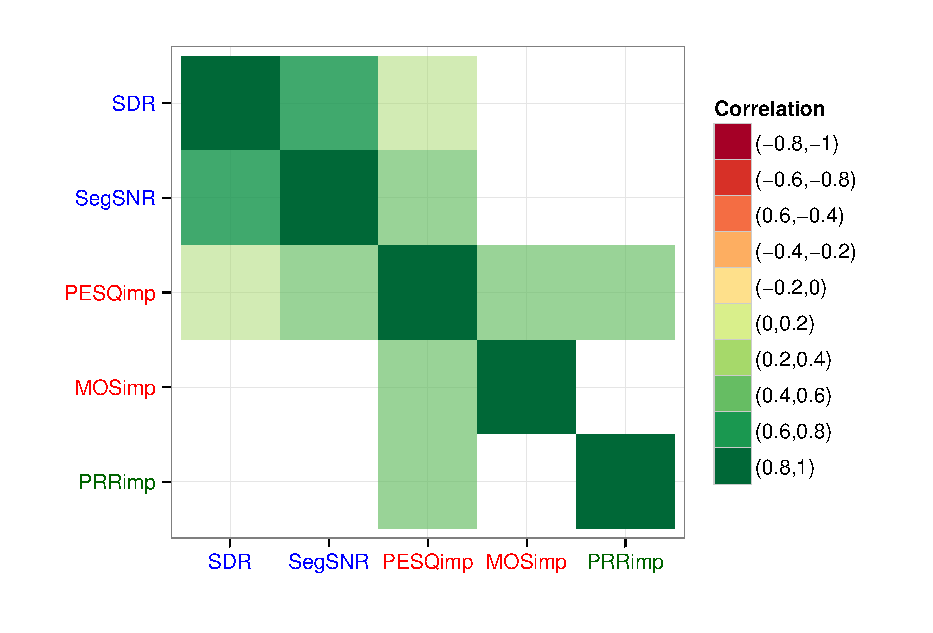
\includegraphics[width=0.7\textwidth]{fig/R/cor/litResCorr}
\par\end{centering}

Highlighted in \textcolor{blue}{blue} are the statistical measures,
\textcolor{red}{red} the human perceptual measures and \textcolor{dkgreen}{green}
the machine recognition measures.

\protect\caption{\label{fig:litResCorr}Pearson's correlation over some of the evaluation
measures}
\end{figure}



\section{Improving Practicality}

The following are the results of investigations attempting to answer
Research Question \ref{enu:ResQ2}, \textit{\RQtwo{}}


\subsection{Investigating Current Training Requirements}

The results of the experiments proposed in \subsecref{Investigating-Training-Req}
are given in this section. \figref{vary-train-moh-pesq} shows the
\ac{PESQ} results of the \ac{BNMF} algorithm developed by \citet{mohammadiha2013supervised}.
Similarly, \figref{vary-train-moh-segsnr} shows the segmental \ac{SNR}
results of the same algorithm.

\begin{figure}[h]
\noindent \begin{centering}
\subfloat[Raw \ac{PESQ} performance]{\noindent \begin{centering}
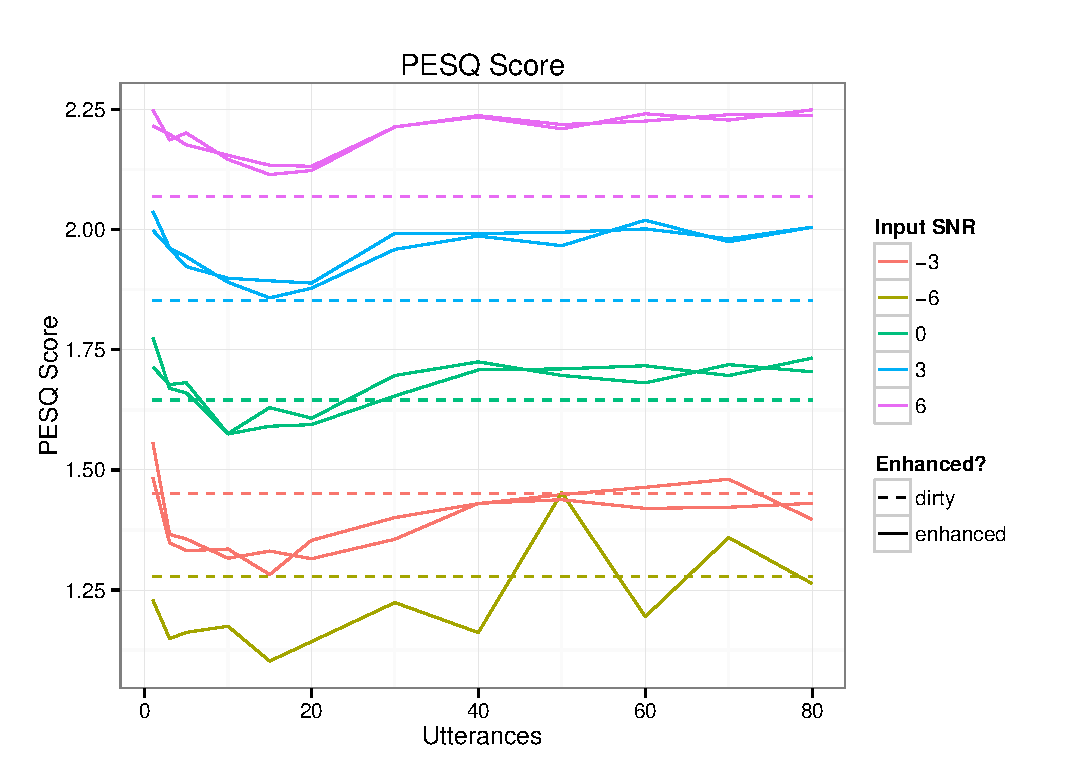
\includegraphics[width=1\textwidth]{fig/R/train/mohSup/pesq}
\par\end{centering}

}
\par\end{centering}

\noindent \begin{centering}
\subfloat[\ac{PESQ} improvement performance]{\noindent \begin{centering}
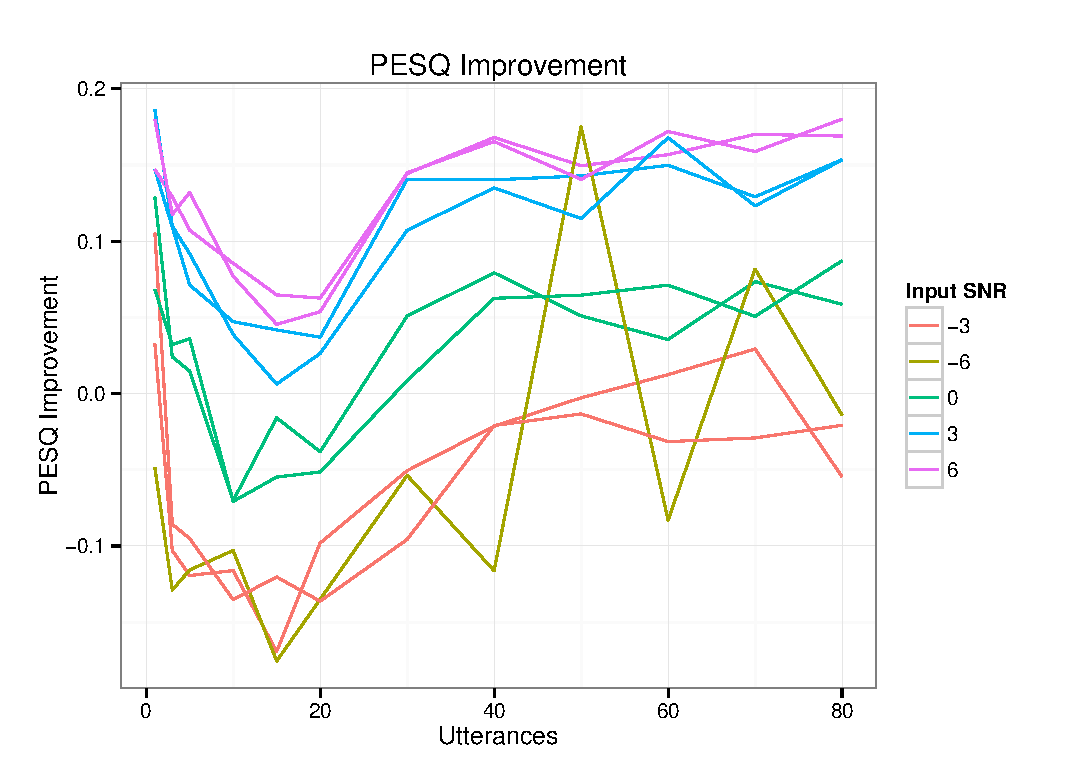
\includegraphics[width=1\textwidth]{fig/R/train/mohSup/pesqImp}
\par\end{centering}

}
\par\end{centering}

\protect\caption{\label{fig:vary-train-moh-pesq}\acs{PESQ} results of \acs{BNMF}
algorithm as training is increased}
\end{figure}


\begin{figure}[h]
\noindent \begin{centering}
\subfloat[Raw segmental \ac{SNR} performance]{\noindent \begin{centering}
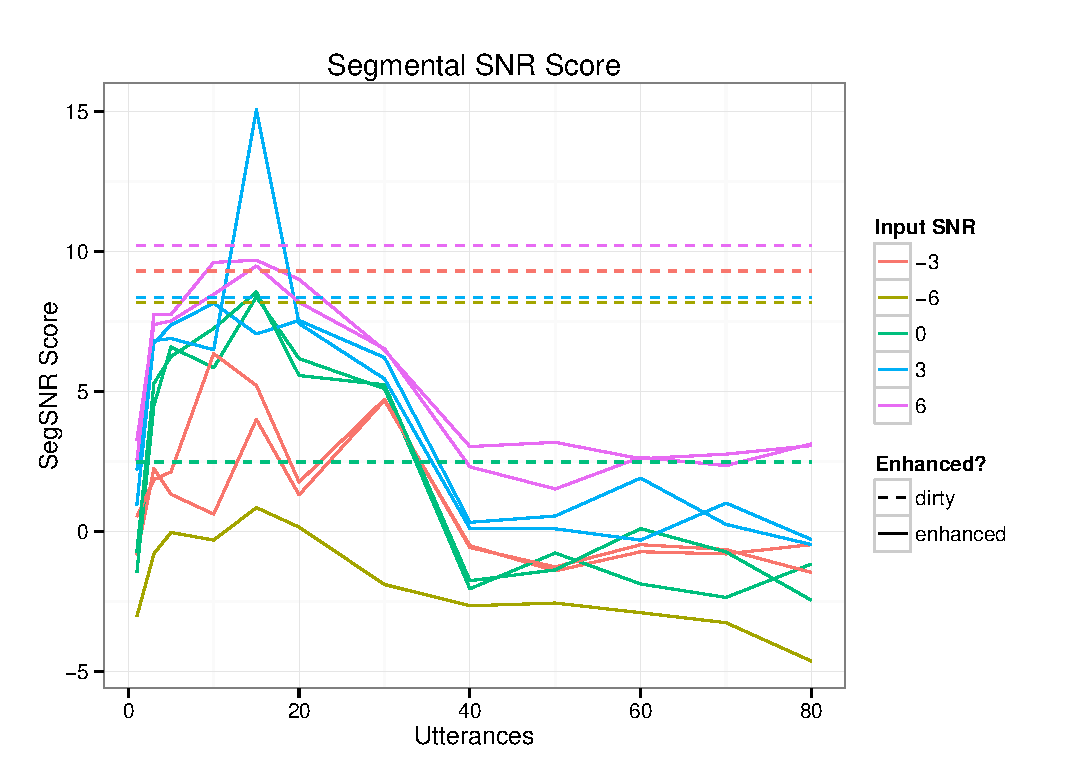
\includegraphics[width=1\textwidth]{fig/R/train/mohSup/segSNR}
\par\end{centering}

}
\par\end{centering}

\noindent \begin{centering}
\subfloat[Segmental \ac{SNR} improvement performance]{\noindent \begin{centering}
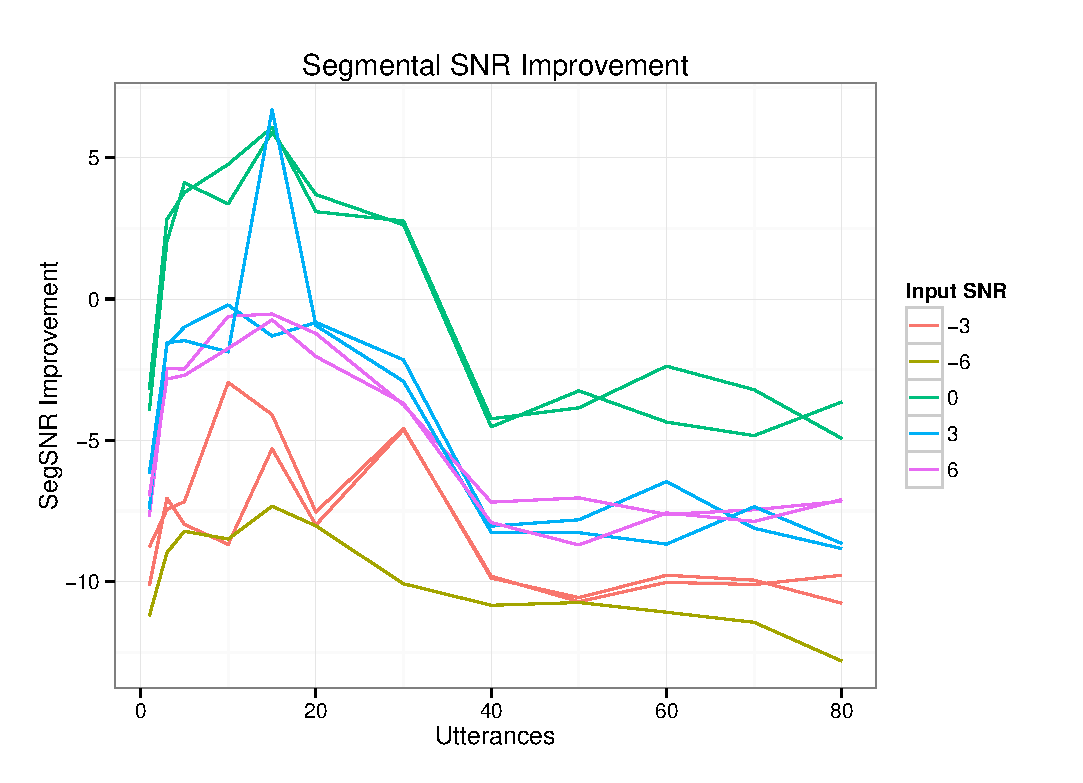
\includegraphics[width=1\textwidth]{fig/R/train/mohSup/segSNRImp}
\par\end{centering}

}
\par\end{centering}

\protect\caption{\label{fig:vary-train-moh-segsnr}Segmental \acs{SNR} results of
\acs{BNMF} algorithm as training is increased}
\end{figure}
\selectlanguage{english}%

